\documentclass{standalone}
\usepackage{tikz}
\begin{document}
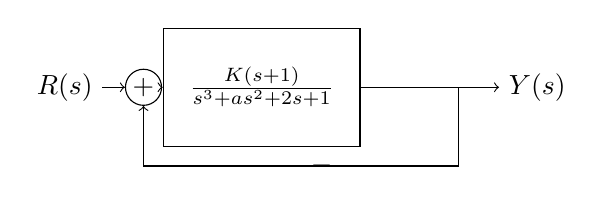
\begin{tikzpicture}
    % Add the block
    \node [draw, rectangle, minimum width=2.5cm, minimum height=1.5cm] (G) at (2.5,0) {$\frac{K(s+1)}{s^3 + a s^2 + 2 s + 1}$};
    
    % Input node
    \node at (0,0) (input) {$R(s)$};
    
    % Output node
    \node at (6,0) (output) {$Y(s)$};
    
    % Sum node
    \node [circle, draw, inner sep=1pt] at (1,0) (sum) {$+$};
    
    % Connections
    \draw[->] (input) -- (sum);
    \draw[->] (sum) -- (G);
    \draw[->] (G) -- (output);
    \draw[->] (5,0) |- ++(0,-1) -| node[pos=0.25, right] {$-$} (sum);
\end{tikzpicture}
\end{document}
